\chapter{Deseño}
\label{app:deseno-detallado}

\section{Wireframes}
\label{app:wireframes}

Nesta sección recóllense os wireframes elaborados durante a fase de deseño, organizados segundo os principais fluxos de interacción da aplicación. A Figura~\ref{fig:wireframes-configuracion} mostra as pantallas asociadas á configuración inicial e á vinculación entre dispositivos; a Figura~\ref{fig:wireframes-paciente} recolle o fluxo de incorporación dunha folla e o acceso á pauta por parte do paciente; a Figura~\ref{fig:wireframes-seguimento} presenta as principais pantallas empregadas para o seguimento do tratamento; e a Figura~\ref{fig:wireframes-supervisor} agrupa as interfaces relacionadas co perfil supervisor e os axustes da aplicación. Finalmente, a Figura~\ref{fig:wireframes-modo-sinxelo-anexo} recolle os wireframes correspondentes ao modo sinxelo.

% ============================================================
% CONFIGURACIÓN INICIAL
% ============================================================

\begin{figure}[h]
    \centering

    \begin{subfigure}[t]{0.23\textwidth}
        \centering
        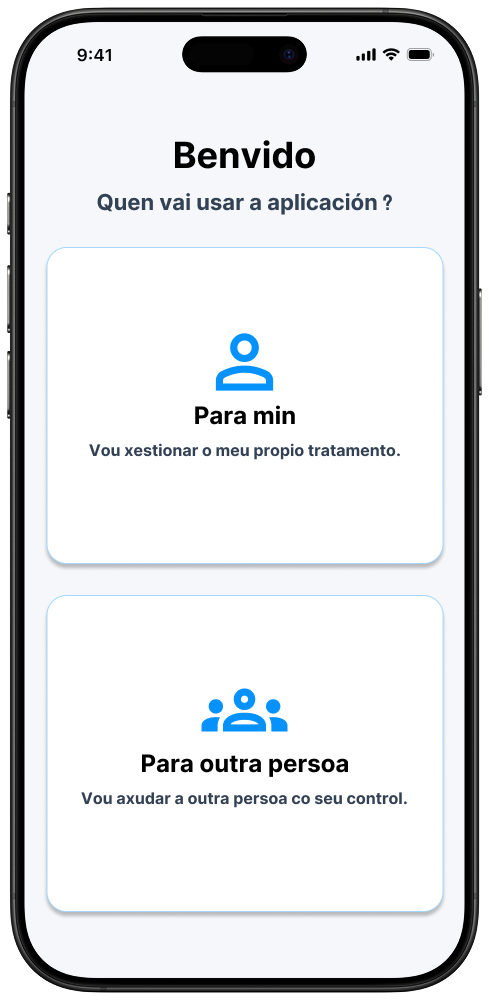
\includegraphics[width=\linewidth]
        {imaxes/07-Deseño/anexo/wireframes/Pantalla setup.png}
        \caption{Selección do rol.}
        \label{fig:wireframe-seleccion-rol}
    \end{subfigure}
    \hfill
    \begin{subfigure}[t]{0.23\textwidth}
        \centering
        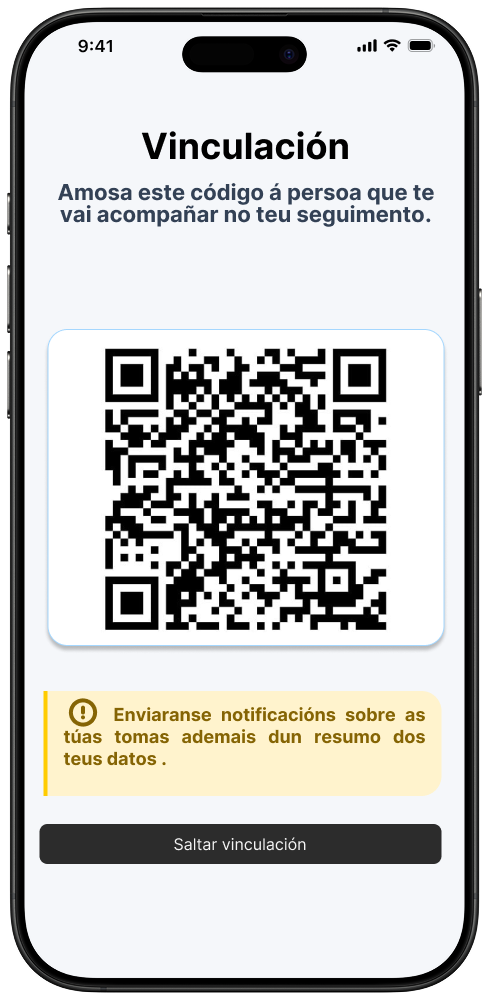
\includegraphics[width=\linewidth]
        {imaxes/07-Deseño/anexo/wireframes/Pantalla setup 2.png}
        \caption{Vinculación do paciente.}
        \label{fig:wireframe-vinculacion-paciente}
    \end{subfigure}
    \hfill
    \begin{subfigure}[t]{0.23\textwidth}
        \centering
        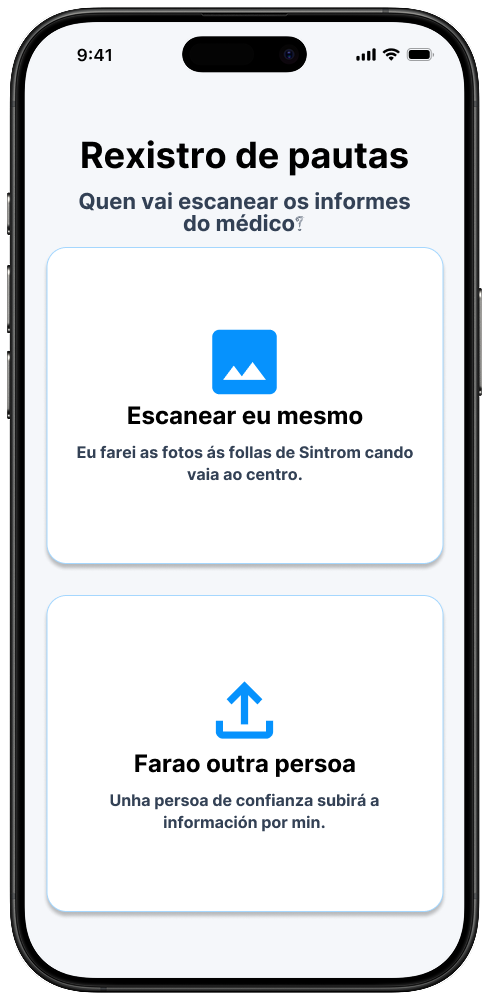
\includegraphics[width=\linewidth]
        {imaxes/07-Deseño/anexo/wireframes/Pantalla setup 3.png}
        \caption{Selección do rexistro das pautas.}
        \label{fig:wireframe-seleccion-rexistro-pautas}
    \end{subfigure}
    \hfill
    \begin{subfigure}[t]{0.23\textwidth}
        \centering
        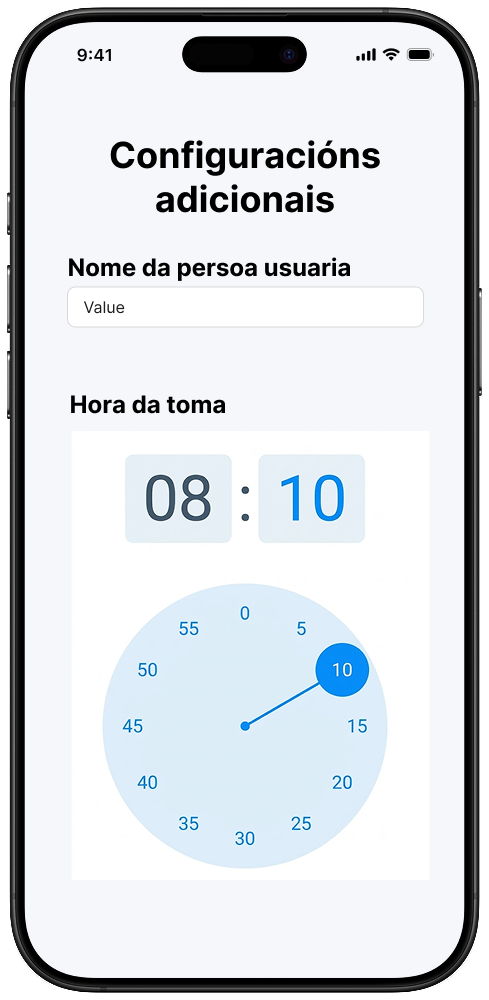
\includegraphics[width=\linewidth]
        {imaxes/07-Deseño/anexo/wireframes/Config adicionais.png}
        \caption{Configuración adicional.}
        \label{fig:wireframe-configuracion-adicional}
    \end{subfigure}

    \caption{Wireframes correspondentes á configuración inicial do paciente.}
    \label{fig:wireframes-configuracion}
\end{figure}


% ============================================================
% INCORPORACIÓN DA FOLLA E PAUTA DO PACIENTE
% ============================================================

\begin{figure}[h]
    \centering

    \begin{subfigure}[t]{0.23\textwidth}
        \centering
        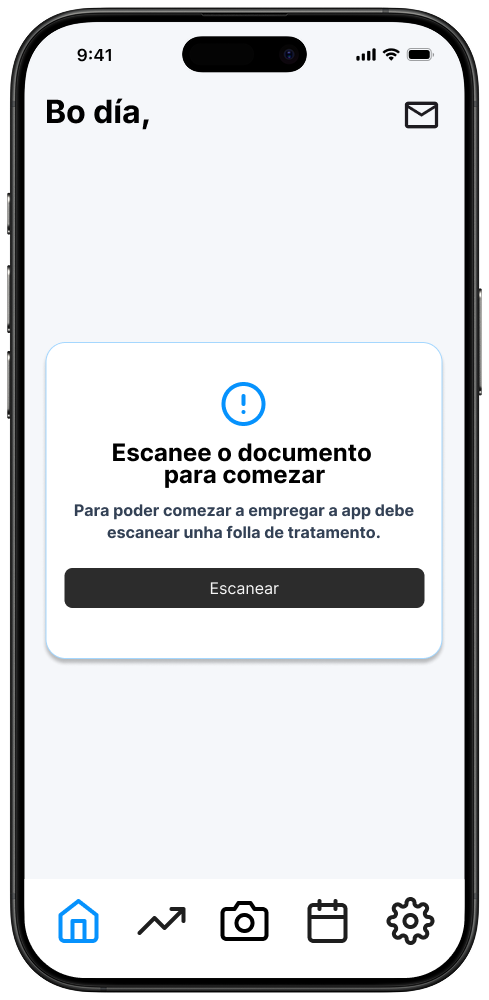
\includegraphics[width=\linewidth]
        {imaxes/07-Deseño/anexo/wireframes/Pantalla inicio vacía.png}
        \caption{Inicio sen pauta.}
        \label{fig:wireframe-inicio-sen-pauta}
    \end{subfigure}
    \hfill
    \begin{subfigure}[t]{0.23\textwidth}
        \centering
        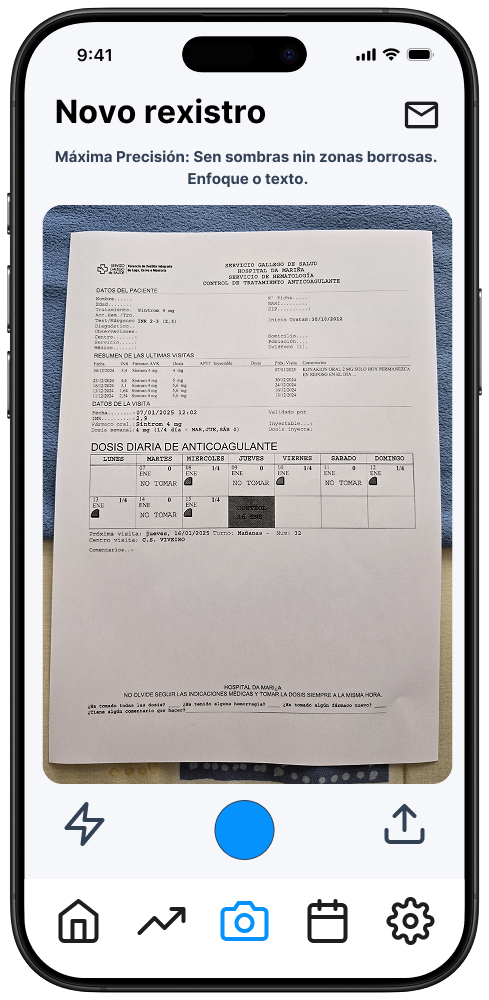
\includegraphics[width=\linewidth]
        {imaxes/07-Deseño/anexo/wireframes/Saca foto.png}
        \caption{Captura da folla.}
        \label{fig:wireframe-captura-folla}
    \end{subfigure}
    \hfill
    \begin{subfigure}[t]{0.23\textwidth}
        \centering
        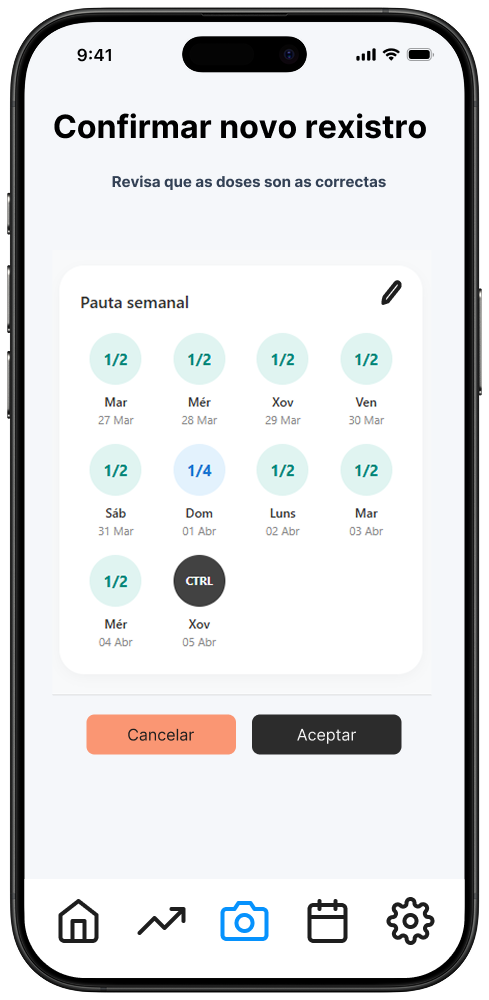
\includegraphics[width=\linewidth]
        {imaxes/07-Deseño/anexo/wireframes/Revisar toma.png}
        \caption{Revisión da pauta.}
        \label{fig:wireframe-revision-pauta}
    \end{subfigure}
    \hfill
    \begin{subfigure}[t]{0.23\textwidth}
        \centering
        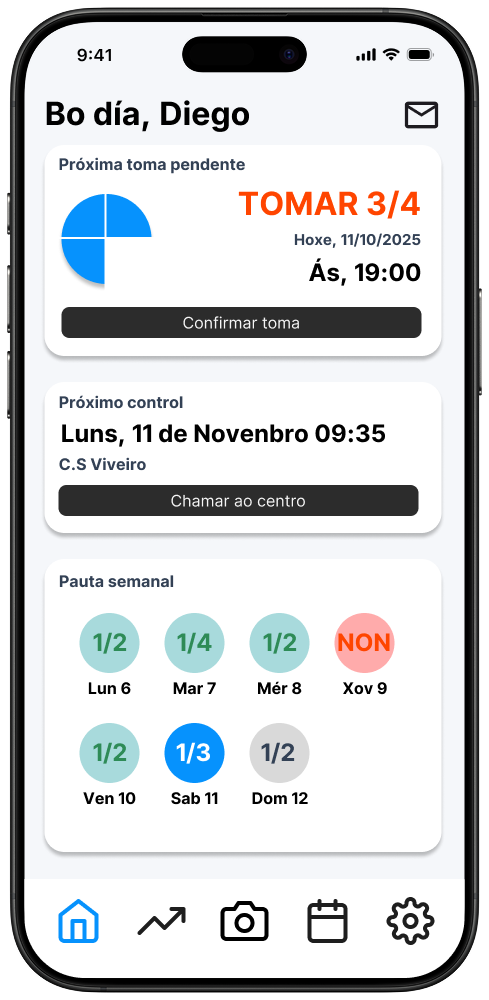
\includegraphics[width=\linewidth]
        {imaxes/07-Deseño/anexo/wireframes/Pantalla inicio.png}
        \caption{Inicio cunha toma pendente.}
        \label{fig:wireframe-inicio-paciente}
    \end{subfigure}

    \caption{Wireframes do fluxo de incorporación dunha folla e presentación da pauta ao paciente.}
    \label{fig:wireframes-paciente}
\end{figure}


% ============================================================
% SEGUIMENTO DO TRATAMENTO
% ============================================================

\begin{figure}[h]
    \centering

    \begin{subfigure}[t]{0.23\textwidth}
        \centering
        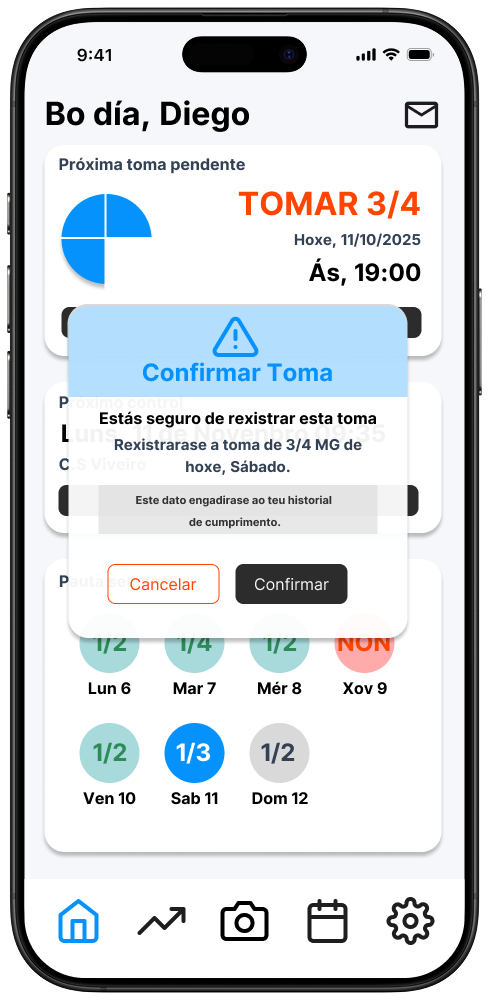
\includegraphics[width=\linewidth]
        {imaxes/07-Deseño/anexo/wireframes/Pantalla inicio Aviso.png}
        \caption{Confirmación dunha toma.}
        \label{fig:wireframe-confirmacion-toma}
    \end{subfigure}
    \hfill
    \begin{subfigure}[t]{0.23\textwidth}
        \centering
        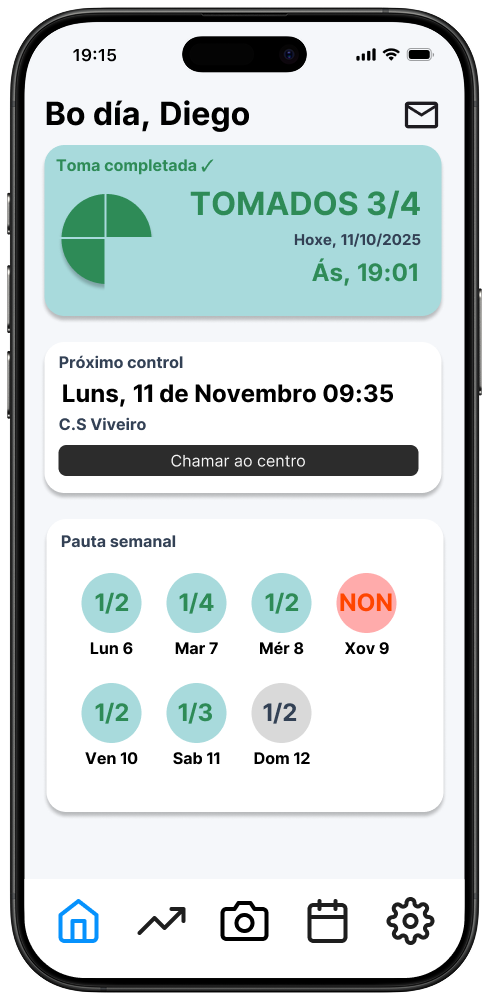
\includegraphics[width=\linewidth]
        {imaxes/07-Deseño/anexo/wireframes/Pantalla inicio 2.png}
        \caption{Toma confirmada.}
        \label{fig:wireframe-inicio-toma-confirmada}
    \end{subfigure}
    \hfill
    \begin{subfigure}[t]{0.23\textwidth}
        \centering
        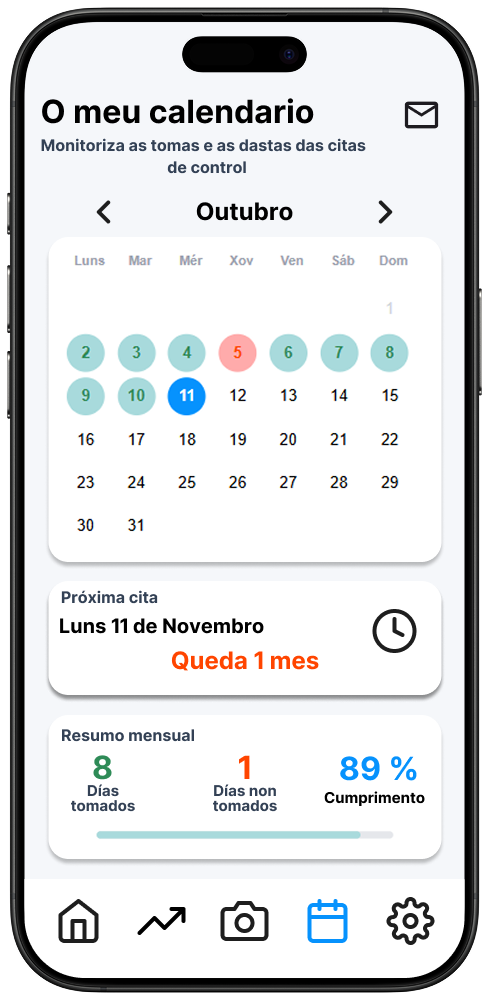
\includegraphics[width=\linewidth]
        {imaxes/07-Deseño/anexo/wireframes/Calendario.png}
        \caption{Calendario.}
        \label{fig:wireframe-calendario}
    \end{subfigure}
    \hfill
    \begin{subfigure}[t]{0.28\textwidth}
        \centering
        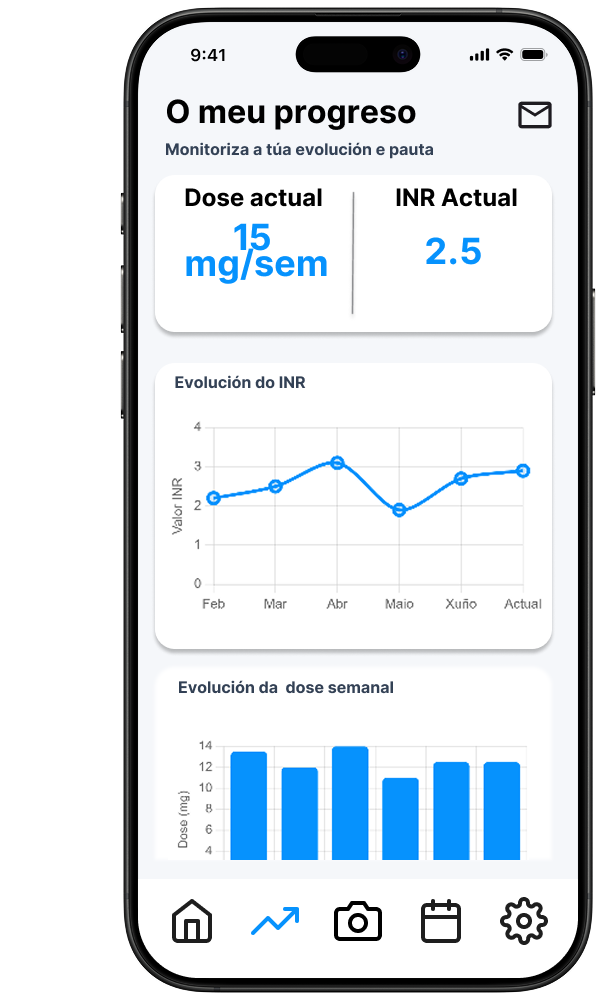
\includegraphics[width=\linewidth]
        {imaxes/07-Deseño/anexo/wireframes/O meu progreso.png}
        \caption{Progreso do tratamento.}
        \label{fig:wireframe-progreso}
    \end{subfigure}

    \caption{Wireframes das principais interfaces de seguimento do tratamento.}
    \label{fig:wireframes-seguimento}
\end{figure}


% ============================================================
% SUPERVISOR E AXUSTES
% ============================================================

\begin{figure}[h]
    \centering

    \begin{subfigure}[t]{0.23\textwidth}
        \centering
        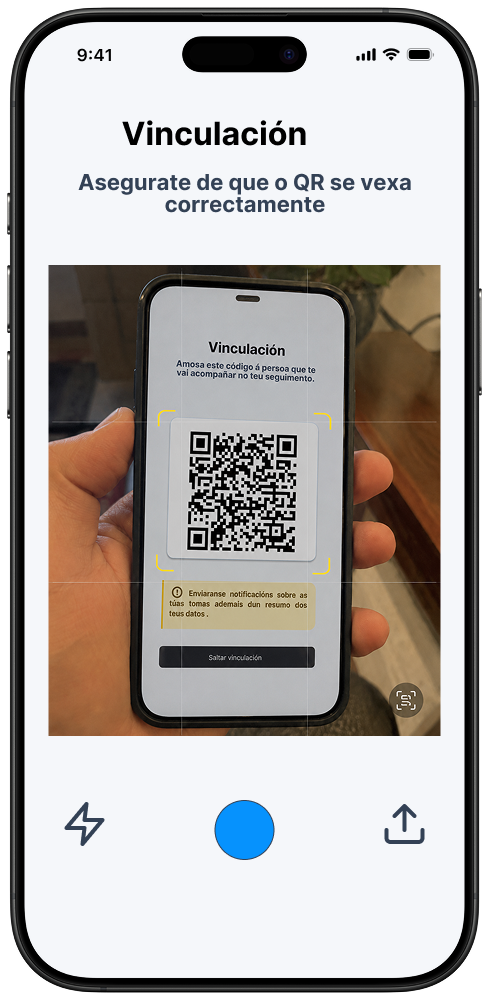
\includegraphics[width=\linewidth]
        {imaxes/07-Deseño/anexo/wireframes/Escaneo QR.png}
        \caption{Escaneo do código QR.}
        \label{fig:wireframe-escaneo-qr}
    \end{subfigure}
    \hfill
    \begin{subfigure}[t]{0.23\textwidth}
        \centering
        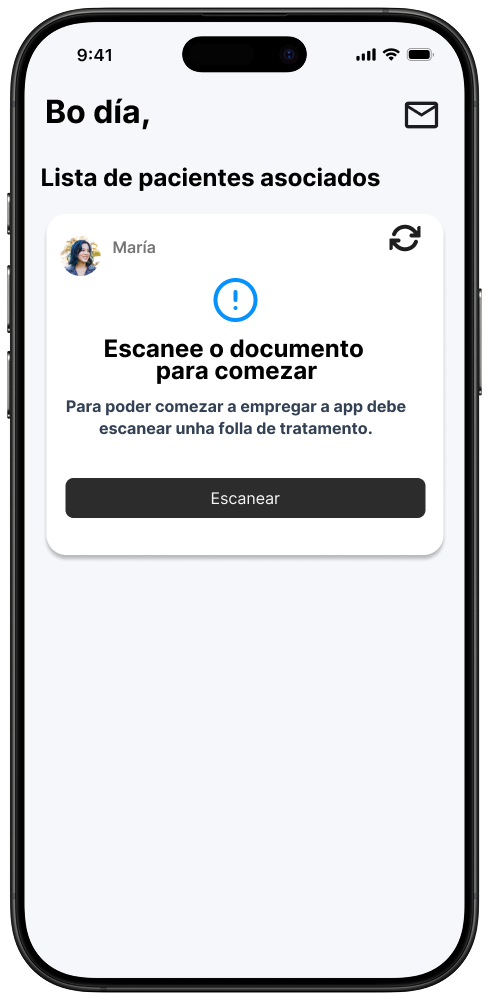
\includegraphics[width=\linewidth]
        {imaxes/07-Deseño/anexo/wireframes/Inicio supervisor.png}
        \caption{Inicio do supervisor.}
        \label{fig:wireframe-inicio-supervisor}
    \end{subfigure}
    \hfill
    \begin{subfigure}[t]{0.24\textwidth}
        \centering
        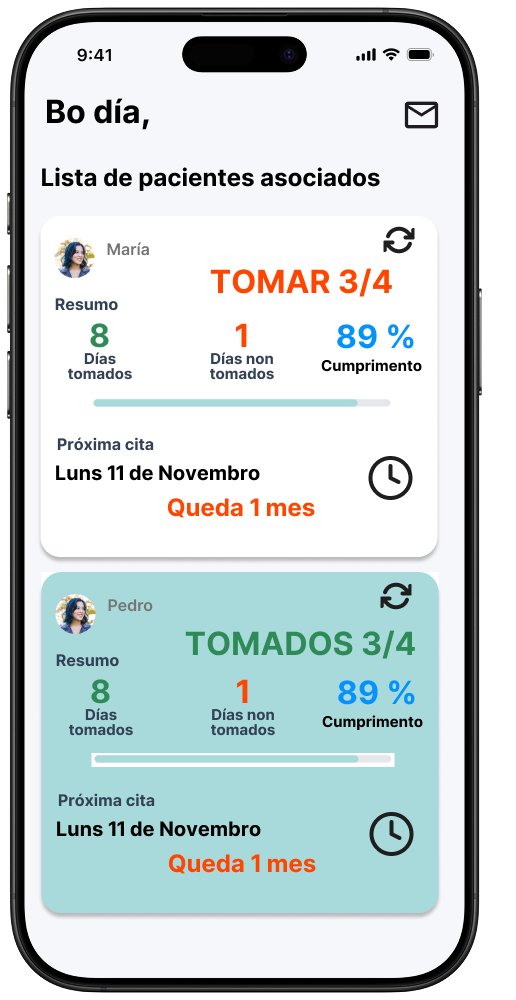
\includegraphics[width=\linewidth]
        {imaxes/07-Deseño/anexo/wireframes/Inicio supervisor toma realizada e varios apcientes.png}
        \caption{Supervisor con varios pacientes.}
        \label{fig:wireframe-inicio-supervisor-varios-pacientes}
    \end{subfigure}
    \hfill
    \begin{subfigure}[t]{0.26\textwidth}
        \centering
        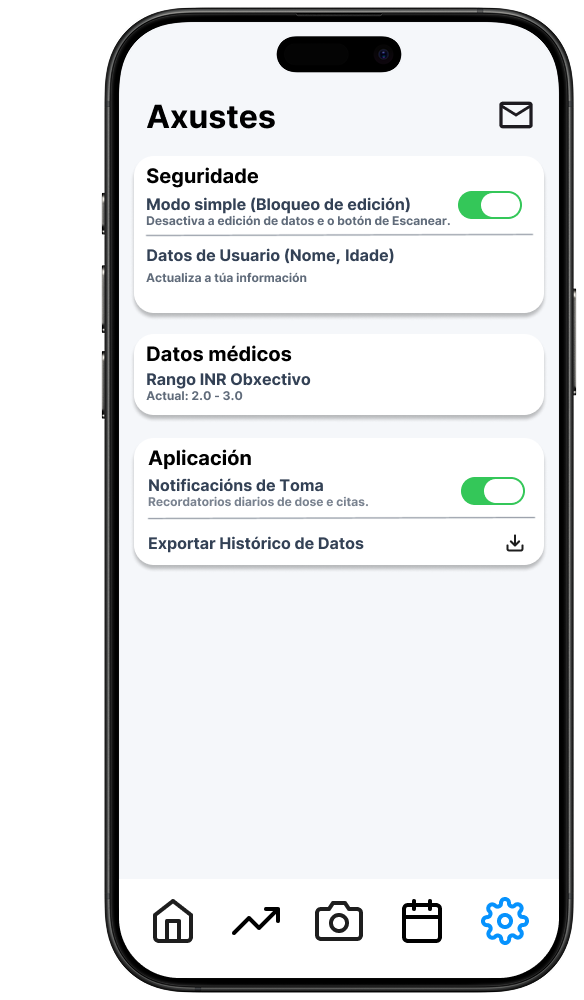
\includegraphics[width=\linewidth]
        {imaxes/07-Deseño/anexo/wireframes/Axustes.png}
        \caption{Axustes da aplicación.}
        \label{fig:wireframe-axustes}
    \end{subfigure}

    \caption{Wireframes do perfil supervisor, da vinculación e dos axustes da aplicación.}
    \label{fig:wireframes-supervisor}
\end{figure}

\begin{figure}[htbp]
    \centering

    \begin{subfigure}[t]{0.23\textwidth}
        \centering
        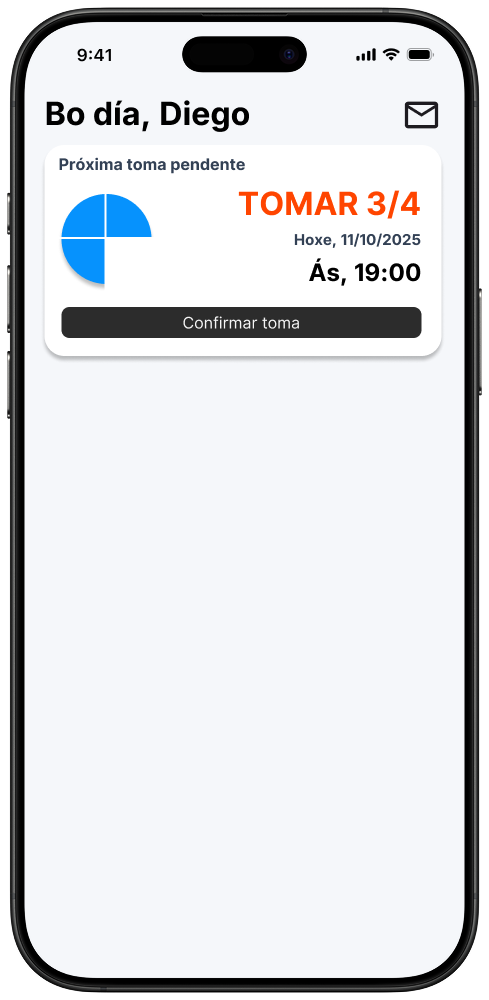
\includegraphics[width=\linewidth]{imaxes/07-Deseño/anexo/wireframes/mock_sinxelo.png}
        \caption{Pantalla principal no modo sinxelo.}
    \end{subfigure}
    \hspace{0.04\textwidth}
    \begin{subfigure}[t]{0.23\textwidth}
        \centering
        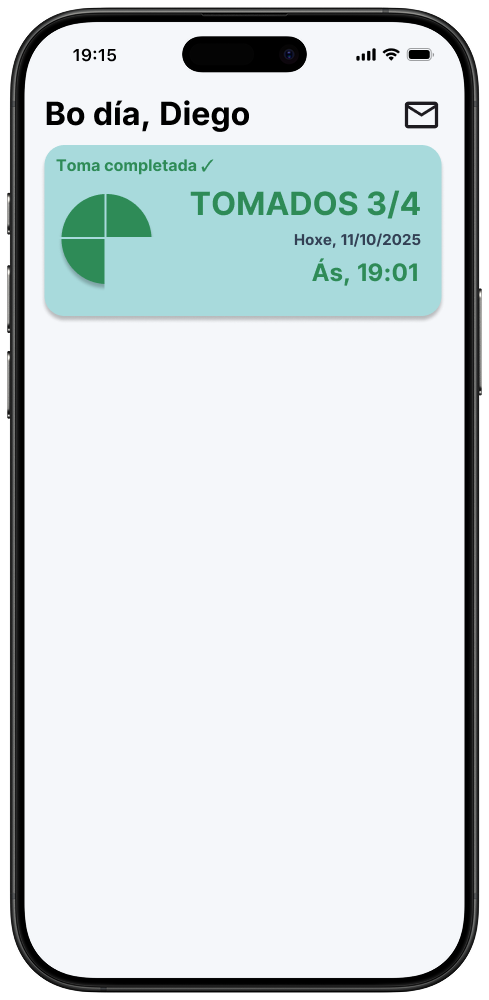
\includegraphics[width=\linewidth]{imaxes/07-Deseño/anexo/wireframes/mock_sinxelo2.png}
        \caption{Acceso aos axustes no modo sinxelo.}
    \end{subfigure}

    \caption{Wireframes correspondentes ao modo sinxelo da aplicación.}
    \label{fig:wireframes-modo-sinxelo-anexo}
\end{figure}